%
%\begin{table}[H]
%    \centering
%    \caption{Testcase matrix. Bold values for the angle of attack (AoA) were provided by Kyle and are considered the maximal attainable values.}
%    \begin{tabular}{ccccccccccc}
%    %\begin{tabular}{lllllllllll}
%        \hline
%        Time [s] & AoA [$^\circ$] & Mach & Re & T [K] & V (m/s) & P [Pa] & $\rho$ [kg/m$^3$] & $\mu$ [Pa$\cdot$s] & $k$ [m$^2$ $\cdot$ s$^{-2}$] & $\omega$ [1/s] \\
%        \hline
%        34.253 & \st{0.31}/\textbf{3.7} & 0.60 & 28608710 & 269.0 & 198.0 & 70970 & 0.918164 & 0.000017 & 10.5 & 13.7 \\
%        43.819 & \st{0.65}/\textbf{3.5} & 0.90 & 27520750 & 255.3 & 289.2 & 53604 & 0.731531 & 0.000016 & 14.0 & 14.7 \\
%        46.477 & \st{0.57}/\textbf{3.4} & 0.99 & 26938250 & 250.5 & 316.0 & 48593.9 & 0.675648 & 0.000016 & 15.3 & 14.8 \\
%        49.400 & \st{0.55}/\textbf{3.4} & 1.10 & 26142750 & 244.9 & 346.7 & 43148.8 & 0.61366 & 0.000016 & 16.8 & 14.8 \\
%        61.624 & \st{0.43}/\textbf{3.4} & 1.67 & 21300900 & 216.7 & 498.2 & 22699.1 & 0.365 & 0.000014 & 25.8 & 13.5 \\
%        107.68 & \st{0.12}/\textbf{2.1} & 4.51 & 511765 & 247.8 & 1423.9 & 325 & 0.00457 & 0.000016 & 118.6 & 0.77 \\
%        \hline
%    \end{tabular}
%    \label{tab:test_matrix}
%\end{table}
%
%\begin{table}[H]
%    \centering
%    \caption{Testcase matrix. Bold values for the angle of attack (AoA) were provided by Kyle and are considered the maximal attainable values.}
%    \begin{tabular}{cccccccccccc}
%        \hline
%        Time [s] & AoA [$^\circ$] & Mach & Re & T [K] & V (m/s) & P [Pa] & $\rho$ [kg/m$^3$] & $\mu$ [Pa$\cdot$s] & $k$ [m$^2$ $\cdot$ s$^{-2}$] & $\omega$ [1/s] & $\delta$ [m] \\
%        \hline
%        34.253 & \textbf{3.7} & 0.60 & 28608710 & 269.0 & 198.0 & 70970 & 0.918164 & 0.000017 & 10.5 & 13.7 & 0.02387 \\
%        43.819 & \textbf{3.5} & 0.90 & 27520750 & 255.3 & 289.2 & 53604 & 0.731531 & 0.000016 & 14.0 & 14.7 & 0.02406 \\
%        46.477 & \textbf{3.4} & 0.99 & 26938250 & 250.5 & 316.0 & 48593.9 & 0.675648 & 0.000016 & 15.3 & 14.8 & 0.02416 \\
%        49.400 & \textbf{3.4} & 1.10 & 26142750 & 244.9 & 346.7 & 43148.8 & 0.61366 & 0.000016 & 16.8 & 14.8 & 0.02431 \\
%        61.624 & \textbf{3.4} & 1.67 & 21300900 & 216.7 & 498.2 & 22699.1 & 0.365 & 0.000014 & 25.8 & 13.5 & 0.02533 \\
%        107.68 & \textbf{2.1} & 4.51 & 511765 & 247.8 & 1423.9 & 325 & 0.00457 & 0.000016 & 118.6 & 0.77 & 0.05338 \\
%        \hline
%    \end{tabular}
%    \label{tab:test_matrix}
%\end{table}
%
%\begin{table}[H]
%    \centering
%    \caption{Testcase matrix. Bold values for the angle of attack (AoA) were provided by Kyle and are considered the maximal attainable values.}
%    \begin{tabular}{cccccccccccc}
%        \hline
%        Time [s] & \textbf{AoA} [$^\circ$] & Mach & Re & T [K] & V [m/s] & P [Pa] & $\rho$ [kg/m$^3$] & $\mu$ [$\mu$Pa$\cdot$s] & $k$ [m$^2$/s$^2$] & $\omega$ [1/s] & $\delta$ [m] \\
%        \hline
%        34.253 & \textbf{3.7} & 0.60 & 28.61M & 269.0 & 198.0 & 70970 & 0.918 & 17 & 10.5 & 13.7 & 0.02387 \\
%        43.819 & \textbf{3.5} & 0.90 & 27.52M & 255.3 & 289.2 & 53604 & 0.732 & 16 & 14.0 & 14.7 & 0.02406 \\
%        46.477 & \textbf{3.4} & 0.99 & 26.94M & 250.5 & 316.0 & 48593.9 & 0.676 & 16 & 15.3 & 14.8 & 0.02416 \\
%        49.400 & \textbf{3.4} & 1.10 & 26.14M & 244.9 & 346.7 & 43148.8 & 0.614 & 16 & 16.8 & 14.8 & 0.02431 \\
%        61.624 & \textbf{3.4} & 1.67 & 21.30M & 216.7 & 498.2 & 22699.1 & 0.365 & 14 & 25.8 & 13.5 & 0.02533 \\
%        107.68 & \textbf{2.1} & 4.51 & 0.51M & 247.8 & 1423.9 & 325 & 0.00457 & 16 & 118.6 & 0.77 & 0.05338 \\
%        \hline
%    \end{tabular}
%    \label{tab:test_matrix}
%\end{table}
%
%\begin{table}[H]
%    \centering
%    \caption{Testcase matrix. Bold values for the angle of attack (AoA) were provided by Kyle and are considered the maximal attainable values.}
%    \begin{tabular}{ccccccccccc}
%        \hline
%        Time [s] & \textbf{AoA} [$^\circ$] & Mach & Re & T [K] & V [m/s] & P [Pa] & $\rho$ [kg/m$^3$] & $\mu$ [$\mu$Pa$\cdot$s] & $k$ [m$^2$/s$^2$] & $\omega$ [1/s] \\
%        \hline
%        34.253 & \textbf{3.7} & 0.60 & 28.61M & 269.0 & 198.0 & 70970 & 0.918 & 17 & 10.5 & 13.7 \\
%        43.819 & \textbf{3.5} & 0.90 & 27.52M & 255.3 & 289.2 & 53604 & 0.732 & 16 & 14.0 & 14.7 \\
%        46.477 & \textbf{3.4} & 0.99 & 26.94M & 250.5 & 316.0 & 48593.9 & 0.676 & 16 & 15.3 & 14.8 \\
%        49.400 & \textbf{3.4} & 1.10 & 26.14M & 244.9 & 346.7 & 43148.8 & 0.614 & 16 & 16.8 & 14.8 \\
%        61.624 & \textbf{3.4} & 1.67 & 21.30M & 216.7 & 498.2 & 22699.1 & 0.365 & 14 & 25.8 & 13.5 \\
%        107.68 & \textbf{2.1} & 4.51 & 511765 & 247.8 & 1423.9 & 325 & 0.00457 & 16 & 118.6 & 0.77 \\
%        \hline
%    \end{tabular}
%    \label{tab:test_matrix}
%\end{table}
%
%\begin{table}[H]
%\centering
%\begin{tabular}{lc}
%\hline
%\textbf{Parameter} & \textbf{Value} \\
%\hline
%Flight Time (s) & 6.162419e+01 \\
%Latitude (deg) & -1.993667e+01 \\
%Longitude (deg) & 1.481571e+02 \\
%Altitude (km) & 1.100024e+01 \\
%Roll (deg) & 0.000000e+00 \\
%Pitch (deg) & 5.447574e+01 \\
%Yaw (deg) & 6.198362e+01 \\
%Omega (x) (Body) & 5.708465e-02 \\
%Omega (y) (Body) & -6.586018e-01 \\
%Omega (z) (Body) & -3.785939e-02 \\
%Velocity x (km/s)(J2000) & -7.463573e-01 \\
%Velocity y (km/s)(J2000) & -3.641400e-01 \\
%Velocity z (km/s)(J2000) & -4.743870e-03 \\
%Thrust (kN)(main engines) & 5.518443e+02 \\
%Mass (tonnes) & 2.125678e+01 \\
%Thrust to Effective Weight ratio & 2.661986e+00 \\
%Mach Number & 1.688090e+00 \\
%AoA (in pitch)(deg) & -2.964313e-01 \\
%AoS(yaw)(deg) & -3.056757e-01 \\
%AoA (total)(deg) & 4.258031e-01 \\
%Dynamic Pressure (Kpa) & 4.527913e+04 \\
%Acceleration with Gravity included (m/s$^2$)(J2000) & 1.593660e+01 \\
%Acceleration without gravity (m/s$^2$)(Body) & 2.281046e+01 \\
%Load Factor Axial & 2.331724e+00 \\
%%Velocity x (m/s)(J2000) & -7.463573e+02 \\
%%Velocity y (m/s)(J2000) & -3.641400e+02 \\
%%Velocity z (m/s)(J2000) & -4.743870e+00 \\
%Static Temperature (K) & 2.167720e+02 \\
%Static Pressure (Pa) & 2.269910e+04 \\
%Density $\rho$ (kg/$m^3$)& 3.647904e-01 \\
%Kinematic Viscosity $\mu$ (Pa $\cdot$ s) & 1.422218e-05 \\
%Reynolds Number & 2.130090e+07 \\
%\hline
%\end{tabular}
%\caption{Flight Parameters and Environmental Conditions}
%\label{tab:eris1.1}
%\end{table}
%
%\begin{figure}[H]
%    \centering
%    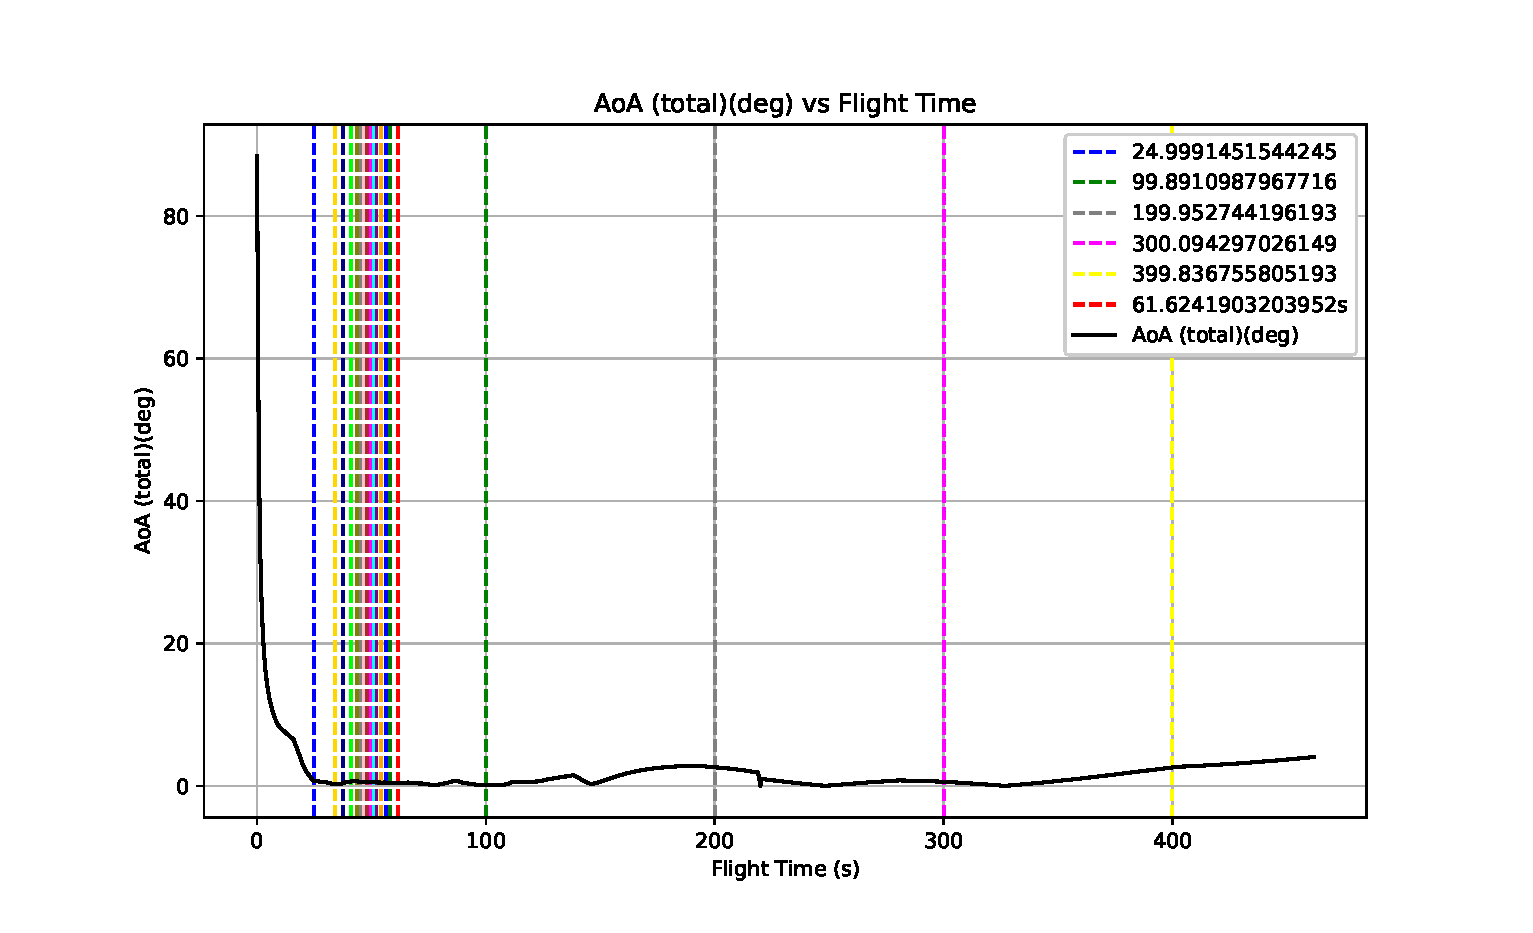
\includegraphics[width=0.495\linewidth]{figs/eris/AoA.eps}
%    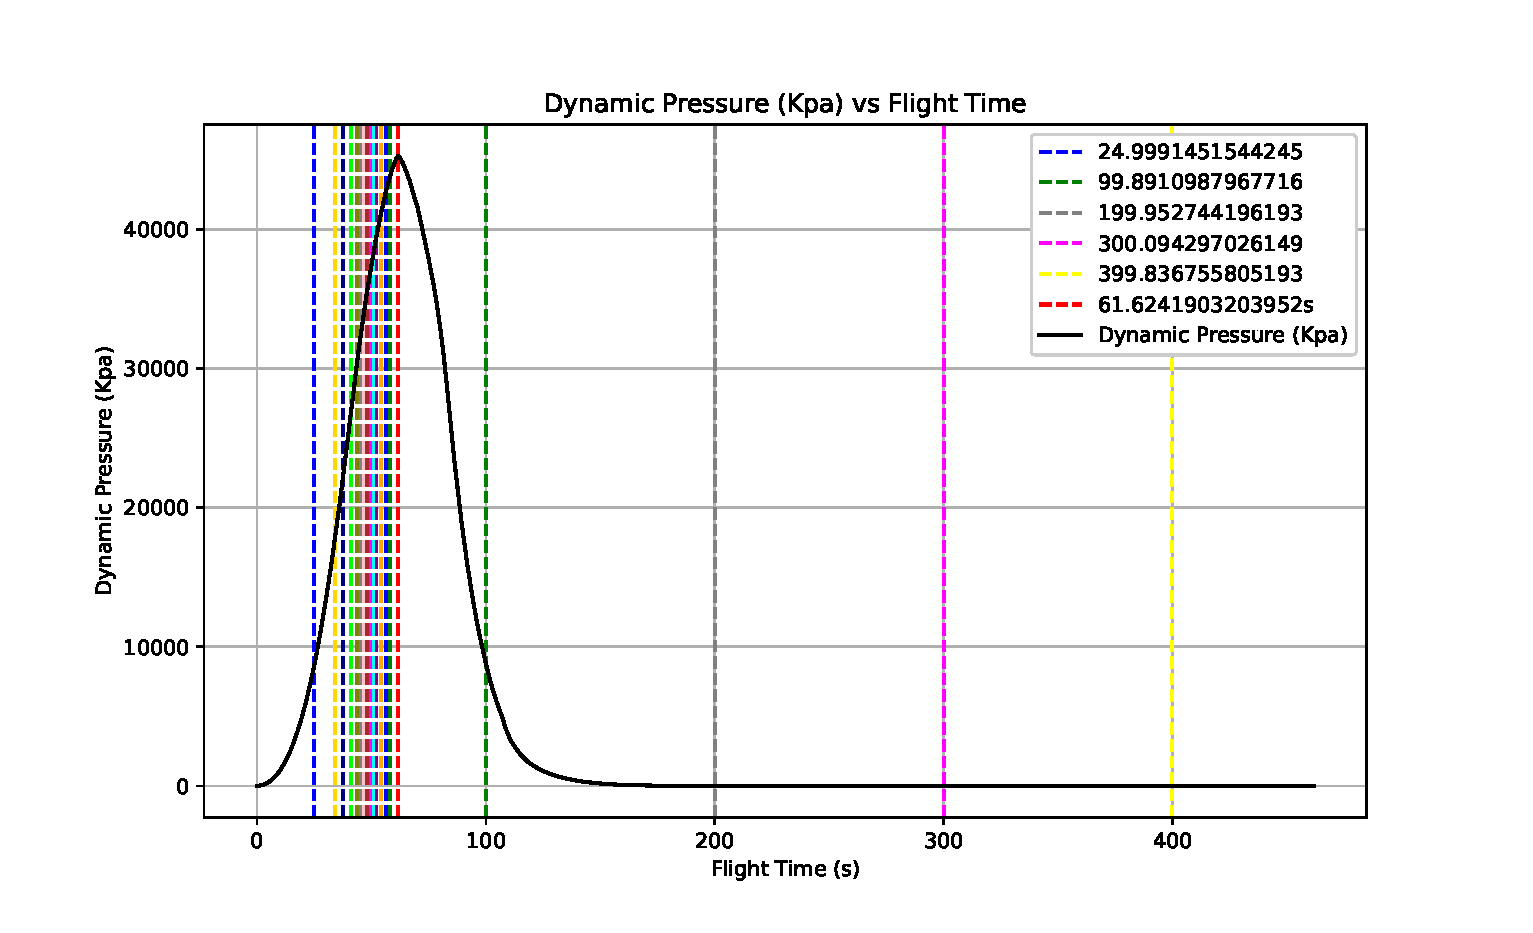
\includegraphics[width=0.495\linewidth]{figs/eris/q.eps}\\
%    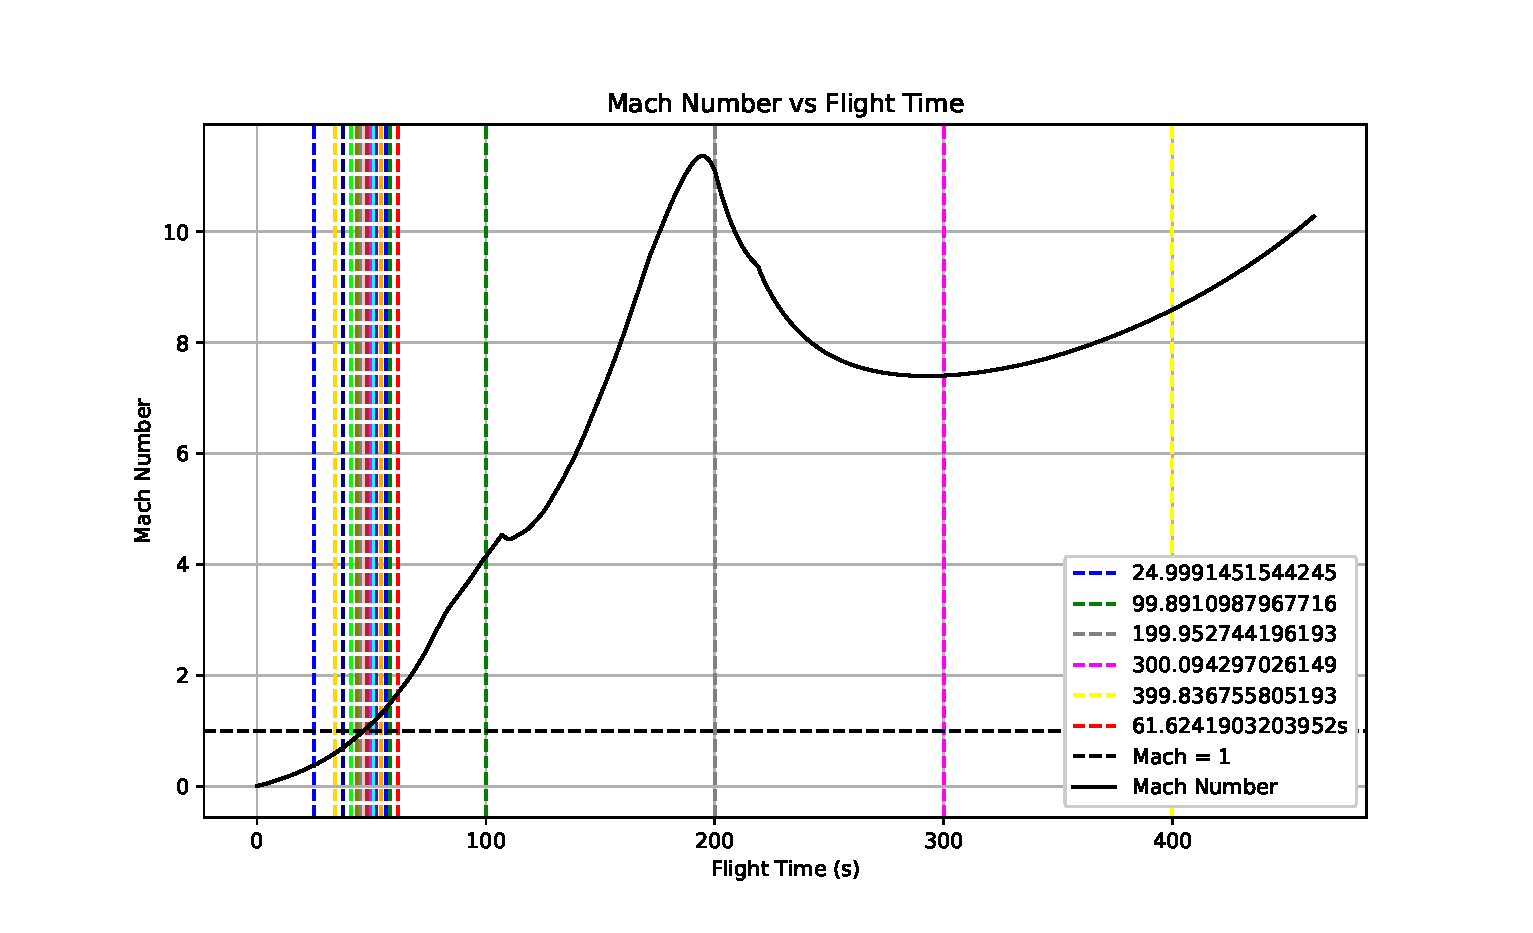
\includegraphics[width=0.495\linewidth]{figs/eris/mach.eps}
%    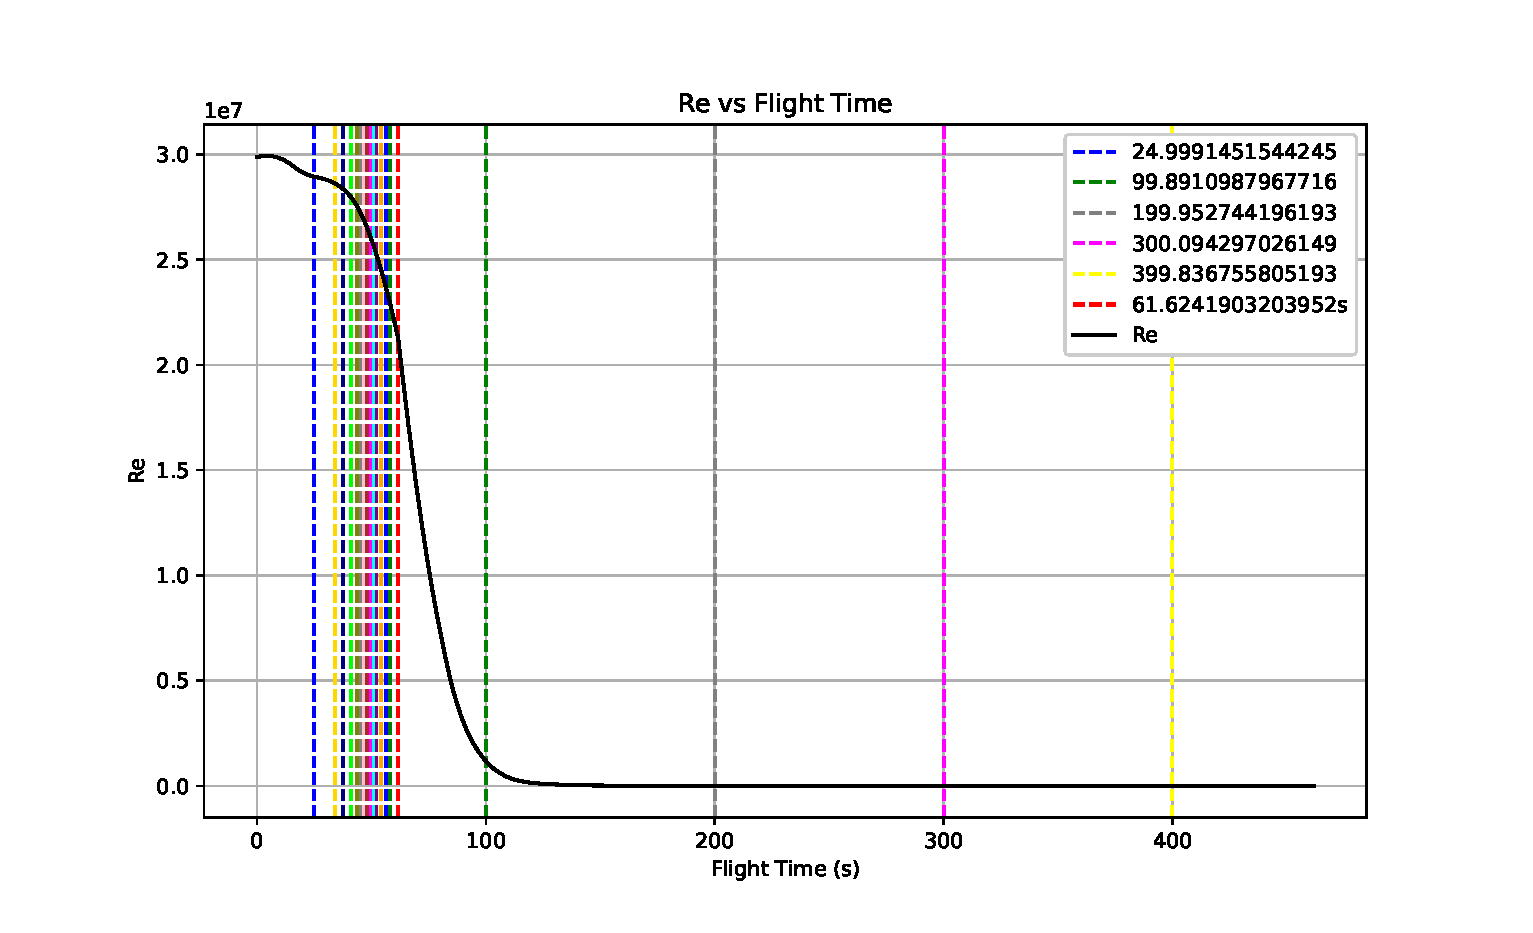
\includegraphics[width=0.495\linewidth]{figs/eris/Re.eps}\\
%    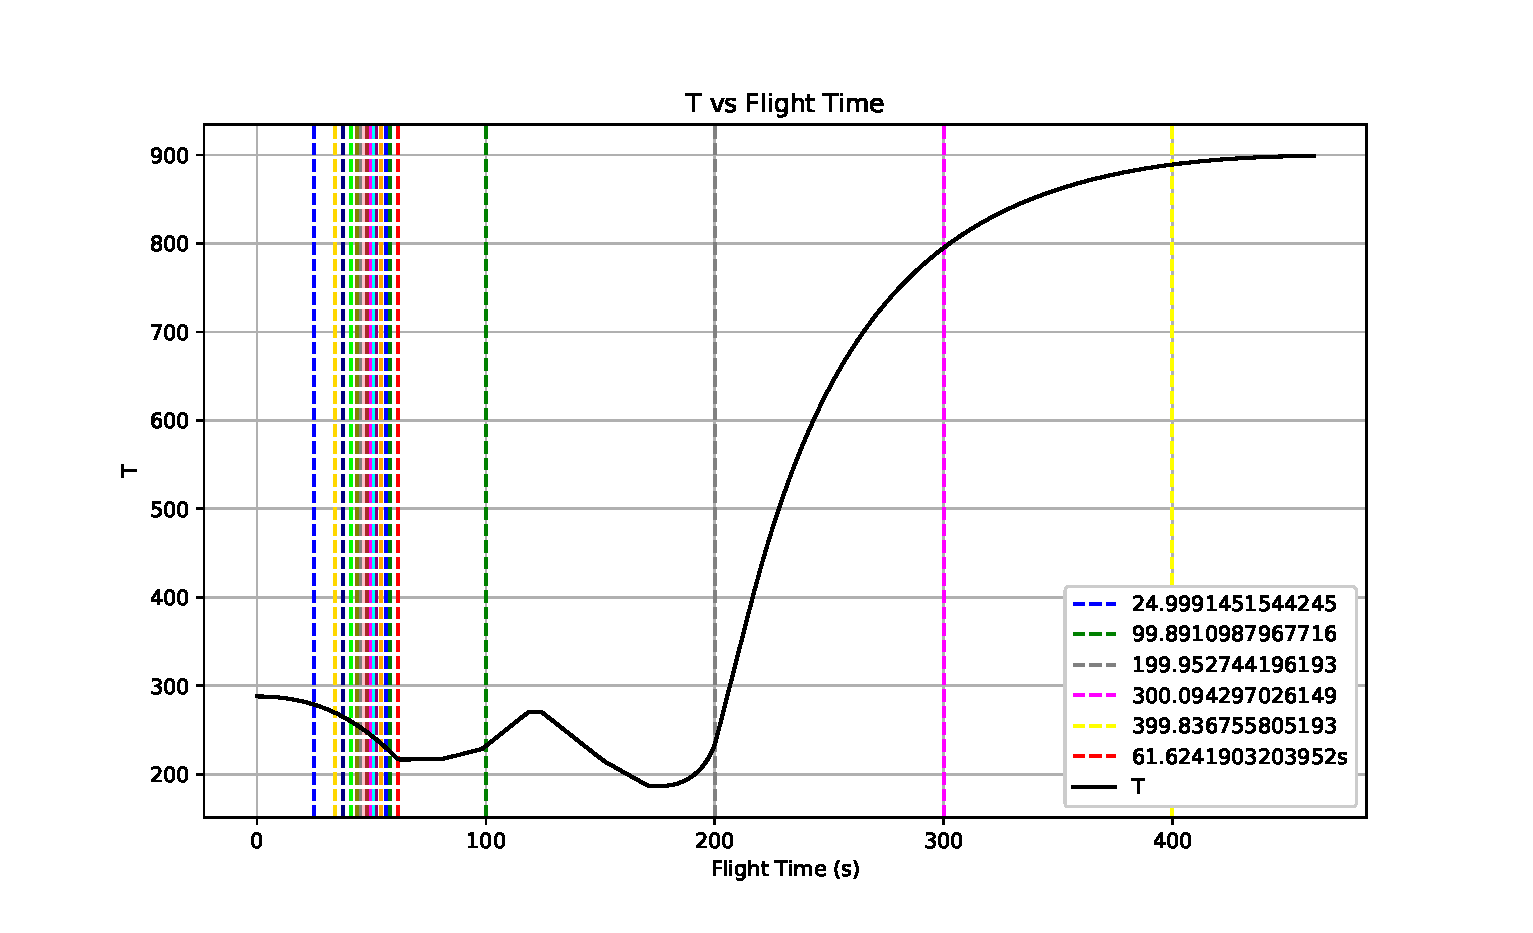
\includegraphics[width=0.495\linewidth]{figs/eris/T.eps}
%    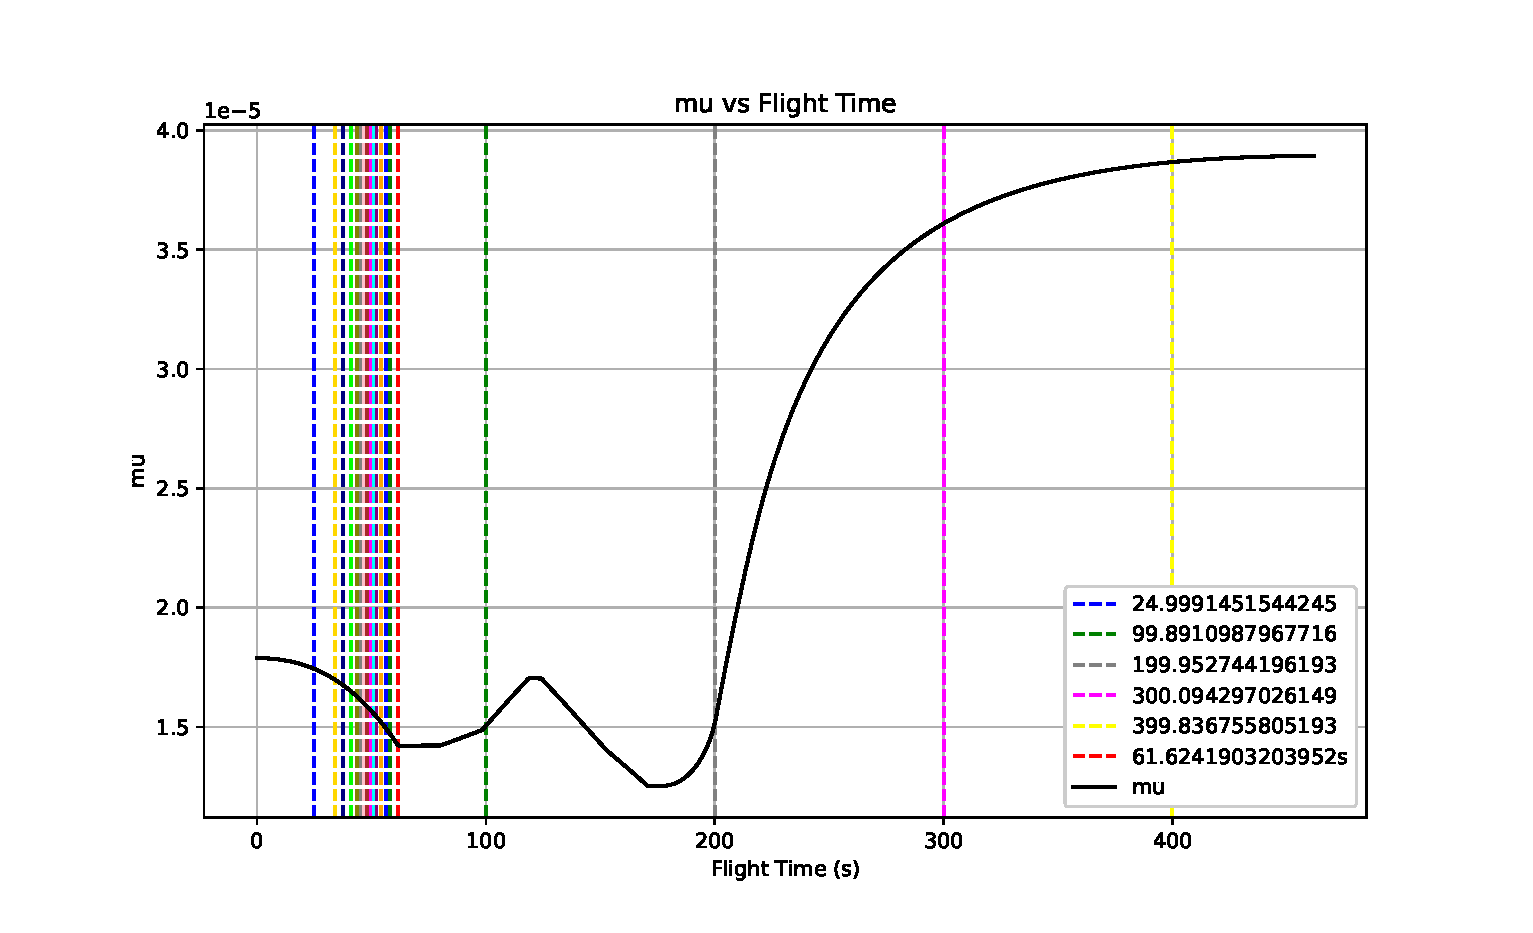
\includegraphics[width=0.495\linewidth]{figs/eris/mu.eps}\\
%    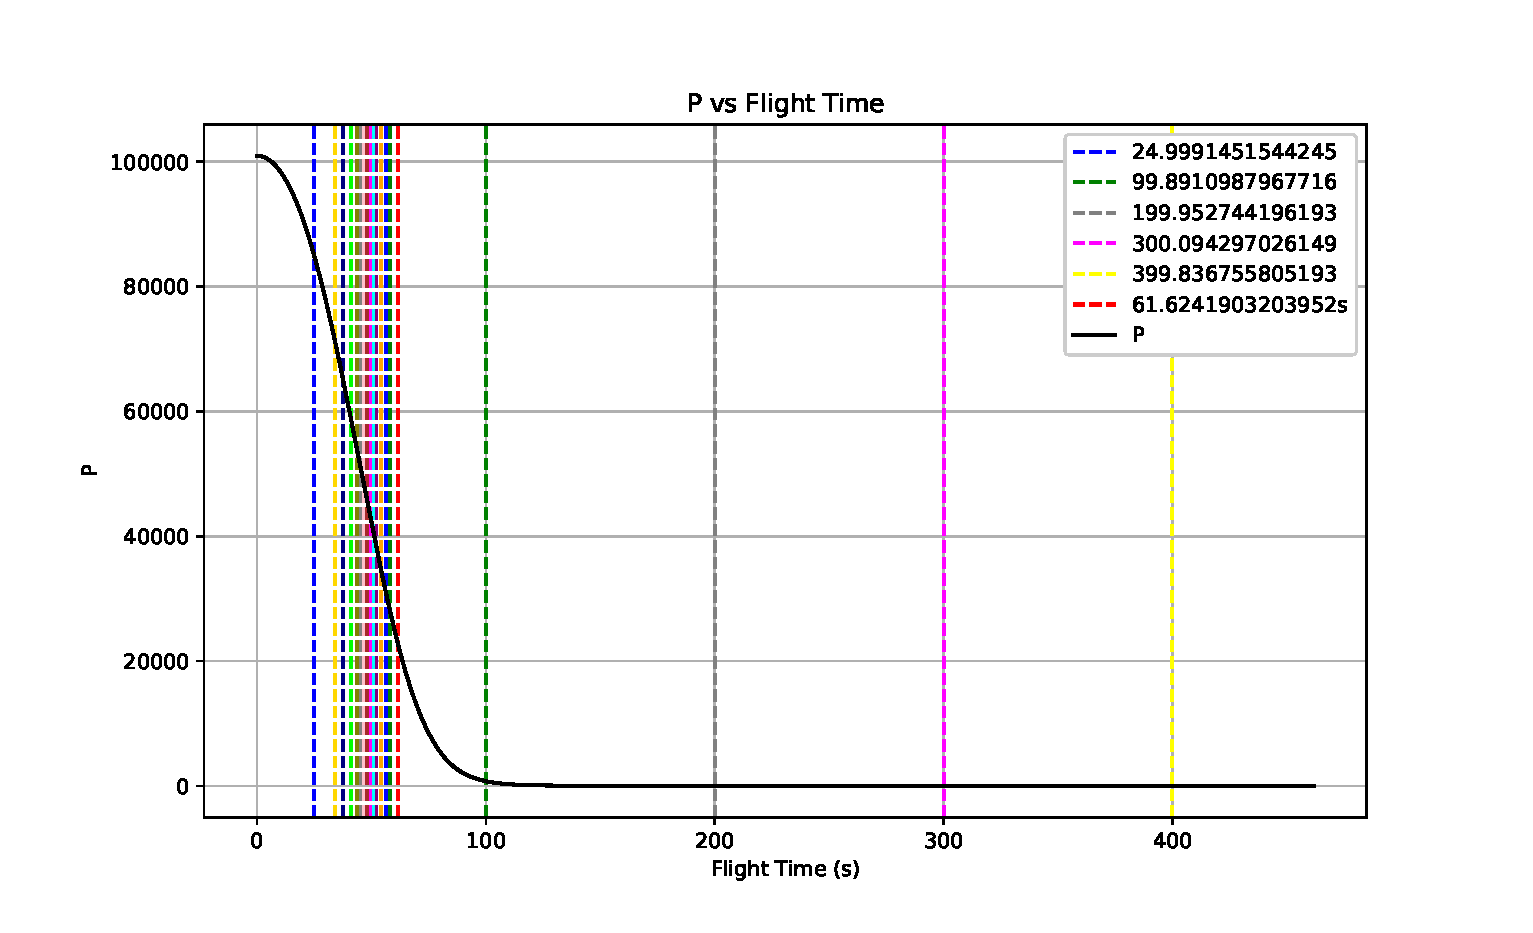
\includegraphics[width=0.495\linewidth]{figs/eris/P.eps}
%    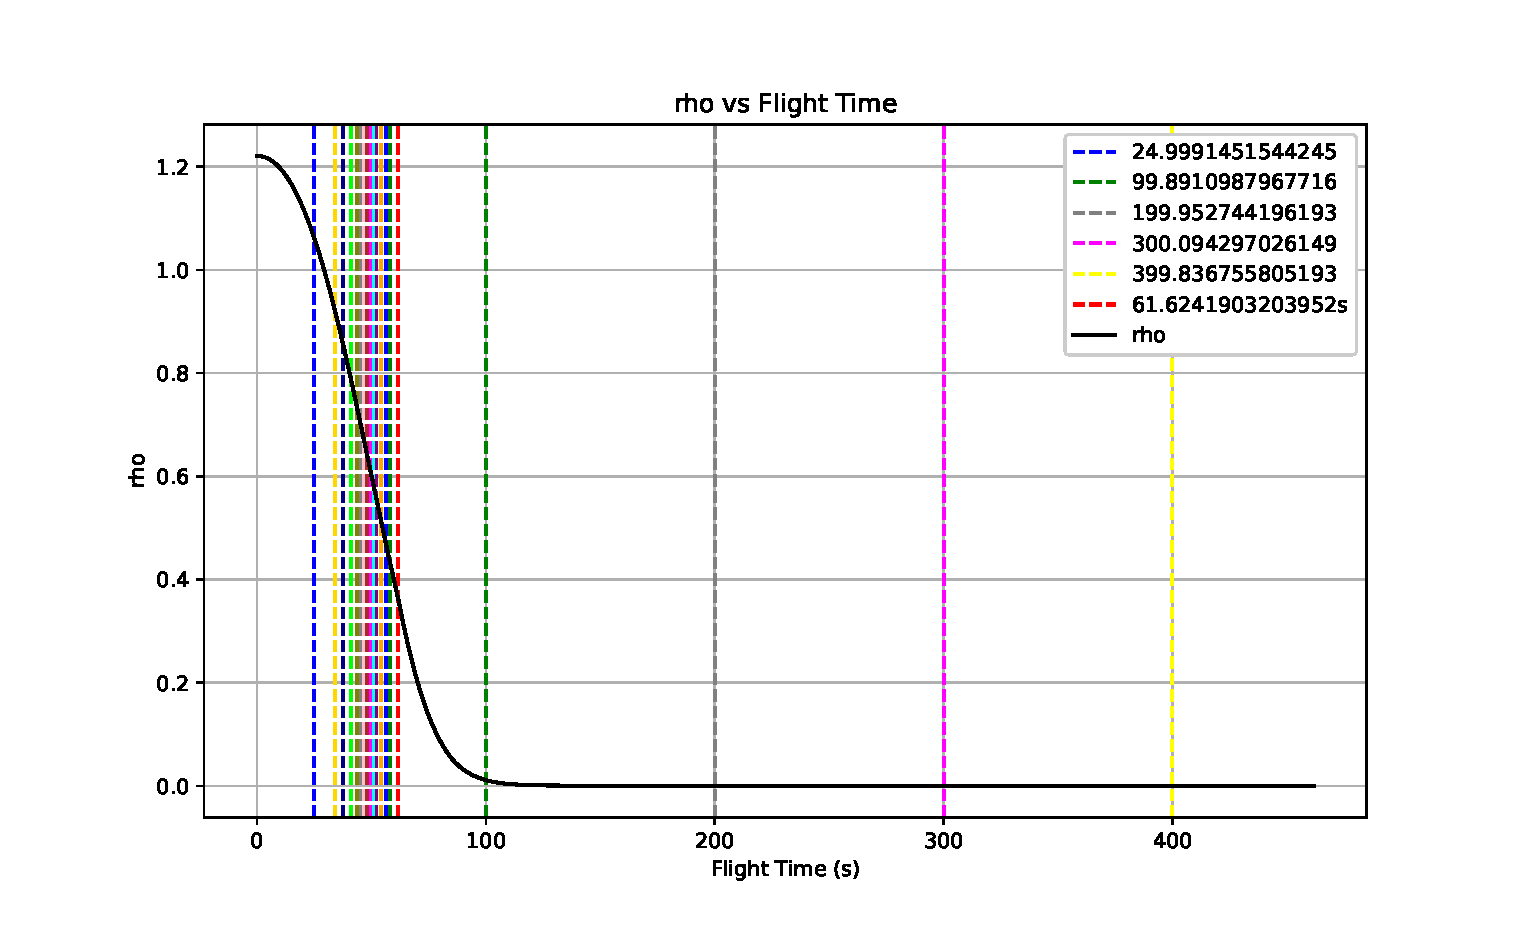
\includegraphics[width=0.495\linewidth]{figs/eris/rho.eps}\\
%    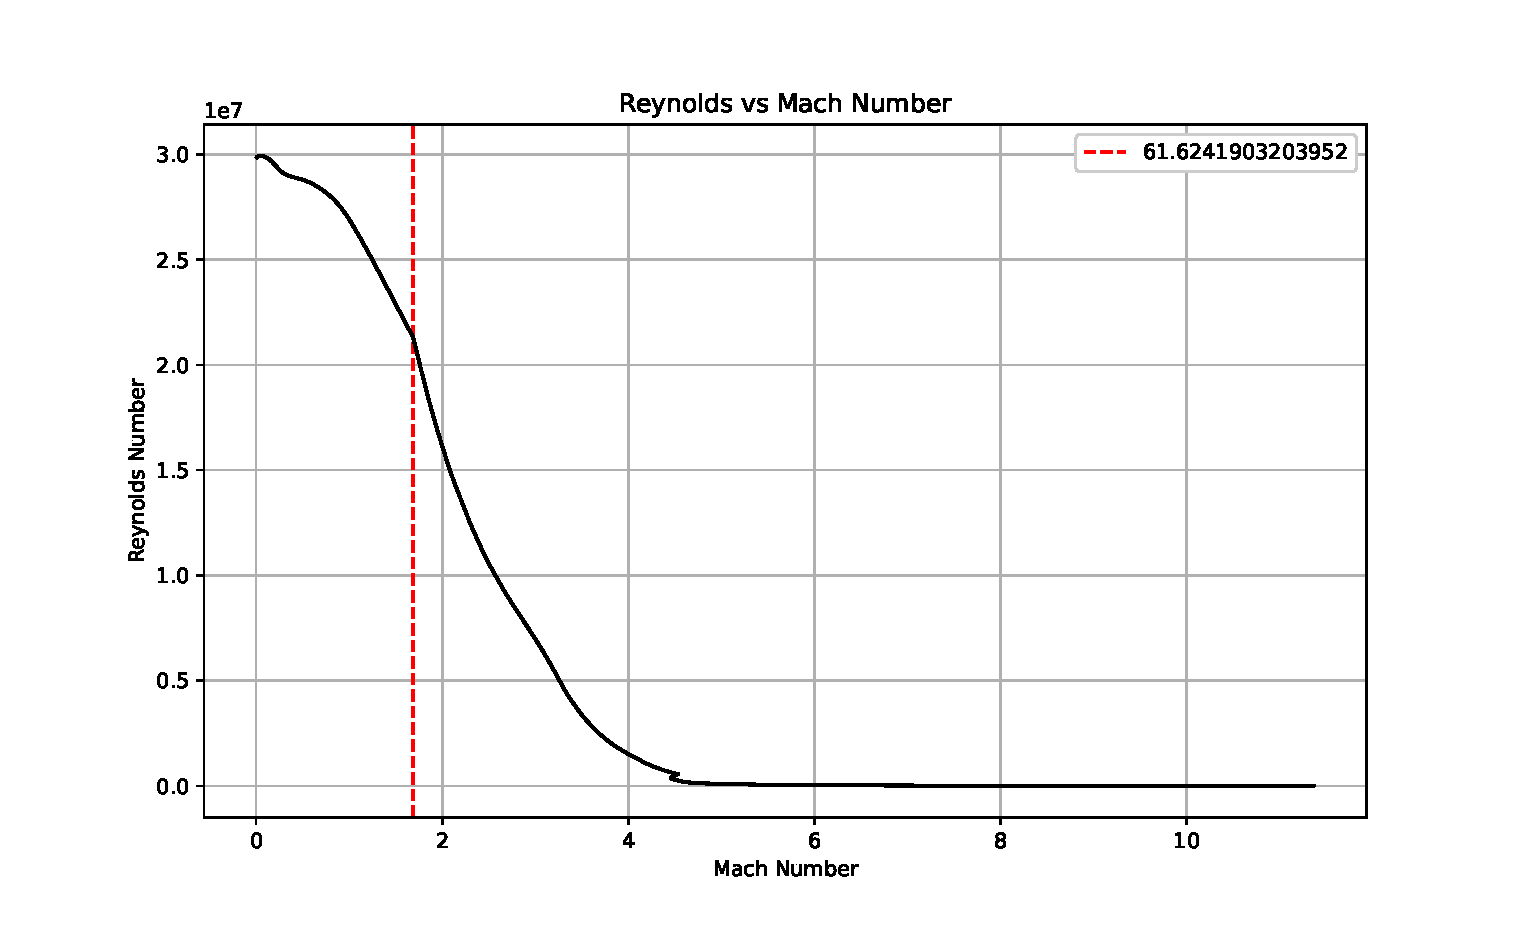
\includegraphics[width=0.495\linewidth]{figs/eris/ReVsMach.eps}
%    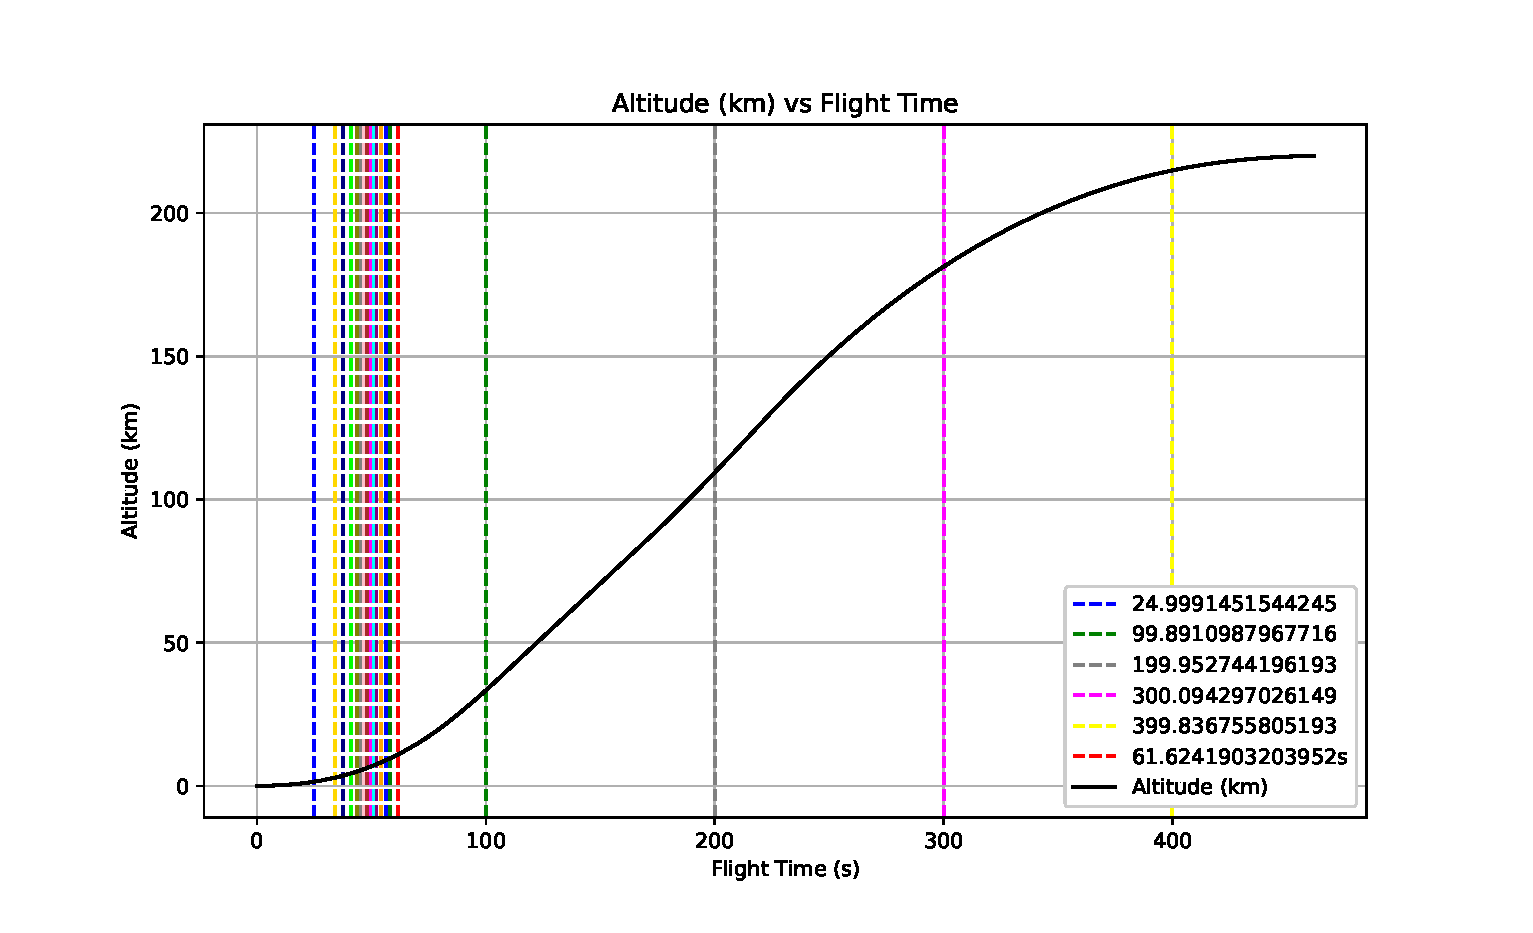
\includegraphics[width=0.495\linewidth]{figs/eris/Altitude.eps}
%    \caption{Trend of several fields in time.}
%    \label{fig:fields}
%\end{figure}